\documentclass{report}

\usepackage[english]{babel}
\usepackage[letterpaper,top=2cm,bottom=2cm,left=3cm,right=3cm,marginparwidth=1.75cm]{geometry}
\usepackage{amsmath}
\usepackage{graphicx}
\usepackage[colorlinks=true, allcolors=blue]{hyperref}

\graphicspath{{images/}}
\title{Getting started with Complex Numbers}

\author{Mr Ashlin Darius Govindasamy\\ \large{University of South Africa}}

\date{\today}

\begin{document}
\pagenumbering{gobble}
\maketitle
\newpage

\tableofcontents

\chapter{Complex Numbers}
\subsection{Introduction to Complex Numbers}
In mathematics, a complex number is an element of a number system that extends the real numbers
with a specific element denoted i, called the imaginary unit and satisfying the equation i²= -1; every
complex number can be expressed in the form a + bi, where a and b are real numbers.

% draw a table of complex numbers i powers
\begin{center}
\begin{tabular}{|c|c|}    
    \hline	
    $i$ & $\sqrt{-1}$ \\ \hline
    $i^2$ & $-1$ \\ \hline
    $i^3$ & $-i$ \\ \hline
    $i^4$ & $1$ \\ \hline
    $i^5$ & $i$ \\ \hline
    $i^6$ & $-i$ \\ \hline
    $i^7$ & $-1$ \\ \hline
    $i^8$ & $i$ \\ \hline
\end{tabular}
\end{center}

% describe table
\begin{center}
    $i$ Chart.
\end{center}

If you look at the table, you can see that the imaginary unit is the $\sqrt{-1}$. Going down the chart you can see there is a pattern till the $i^n$ where $n$ is the power of the imaginary unit.

Remember at least the first 4 powers of the imaginary unit. Later we will use it to evaluate the complex numbers into the form $a+bi$.

\subsection{Graphing Complex Numbers}
In mathematics, the complex plane is the plane formed by the complex numbers, with a Cartesian coordinate system such that the x-axis, called real axis, is formed by the real numbers, and the y-axis, called imaginary axis, is formed by the imaginary numbers. 


% show image
\begin{figure}[h!]
    \centering
    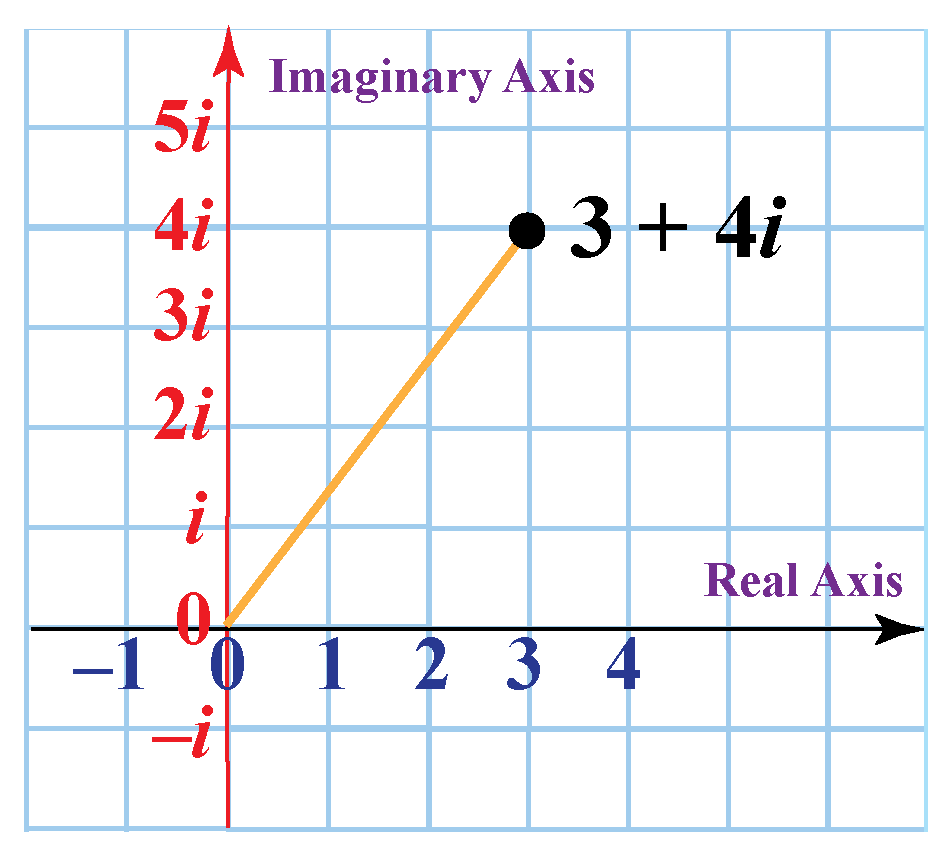
\includegraphics[width=0.35\textwidth]{graphingcomplexnumbers.png}
    \caption{Complex plane}    
\end{figure}

I will come back to this later. We will use this tool in converting standard complex numbers into the polar form $r$ and $\theta$.


\subsection{Operations with Complex Numbers}

\subsubsection{Addition}

To add two complex numbers, add the real part to the real part and the imaginary part to the imaginary part.

\begin{equation}
    (a+bi)+(c+di)=(a+c)+(b+d)i
\end{equation}

Example: $(2+7i)+(3-4i)$

\begin{equation}
    (2+7i)+(3-4i)=(2+3)+(7+(-4))i
    =5+3i
\end{equation}

\subsubsection{Subtraction}
To substract two complex numbers, substract the real part to the real part and the imaginary part to the imaginary part.

\begin{equation}
    (a+bi)-(c+di)=(a-c)+(b-d)i     
\end{equation}

Example: $(2+7i)-(3-4i)$

\begin{equation}
    (2+7i)-(3-4i)=(2-3)+(7+4i)i
    =5+(-3)i
\end{equation}

\subsubsection{Multiplication}
Multiplication of two complex numbers is defined as:
\begin{equation}
    (a+bi)(c+di)=(ac-bd)+(ad+bc)i
\end{equation}

Example: $(2+7i)(3-4i)$

\begin{equation}
    \begin{split}        
(2+7i)(3-4i)=(2*3-4*7)+(2*4+7*3)i\\
=(-10+28)+(12+(-7))i \\
=18+(-7)i            
    \end{split}
\end{equation}

\subsubsection{Conjugate}
Conjugate of a complex number is defined as:
\let\conjugatet\overline
\begin{equation}
    \begin{split}
        \conjugatet{(a+bi)}=a-bi\\
    \end{split}
\end{equation}

Example: $\conjugatet{(2+7i)}$

\begin{equation}
    \begin{split}
        \conjugatet{(2+7i)}=2-7i
    \end{split}
\end{equation}

\begin{center}
    Notice that only the sign between the real and imaginary part is changed oppositely.
\end{center}

\subsubsection{Division}
Division of two complex numbers is defined as:
\begin{equation}
    \begin{split}
    \frac{(a+bi)}{(c+di)} = \frac{(a+bi)(c-di)} {(c+di)(c-di)}\\
    = \frac{(a+bi)(c-di)} {(c^2+d^2)}\\
    = \frac{(a+bi)}{(c^2+d^2)} + \frac{(c-di)}{(c^2+d^2)}i\\    
    \end{split}
\end{equation}

Example: $\frac{(2+7i)}{(3-4i)}$

\begin{equation}
    \begin{split}
    \frac{(2+7i)(3+4i)}{(3-4i)(3+4i)} = \frac{-22+29i}{25}
    = -\frac{22}{25} + \frac{29}{25}i
    \end{split}
\end{equation}



\subsubsection{Modulus}
Finding the modulus of a complex number. \\\\
General formula for Modulus of $a+bi$ is:
\begin{equation}
    \sqrt{a^2+b^2}
\end{equation}

Example : Find the modulus of -4 + 3i.

\begin{equation}
    Modulus = \sqrt{(-4)^2+(3)^2}=\sqrt{25}=5
\end{equation}

\subsection{Computing $i^n$ Complex Numbers}

Remember the first 4 powers of the imaginary unit now we are going to use it to evaluate the complex numbers.

Example: Evaluate $i^{105}$

\begin{equation}
    \begin{split}
        i^{105} = i^{104}*i \\
        i^{104} = (i^2)^{54} \\
        i^{104} = (-1)^{54} = 1\\
        \therefore i^{105} = i
    \end{split}
\end{equation}

Example: Evaluate $i^{647}$
\begin{equation}
    \begin{split}
        i^{647} = i^{646}*i \\
        i^{646} = (i^2)^{323} \\
        i^{646} = (-1)^{323} = -1\\
        \therefore i^{647} = -i
    \end{split}
\end{equation}

Example: Evaluate $i^{142}$
\begin{equation}
    \begin{split}
        i^{142} = (i^2)^{71} \\
        i^{142} = (-1)^{71} = -1\\        
        \therefore i^{142} = -1
    \end{split}
\end{equation}

Bonus: Evaulating $(-1)^n$.

\begin{equation}
    (-1)^n =
    \left\{
        \begin{array}{lr}
            1, & \text{if } n \in \{n=2n | n \in \mathbb{N} \} \\
            -1, & \text{if } n \in \{n=2n+1 | n \in \mathbb{N} \}
        \end{array}
    \right\} 
\end{equation}

\subsection{Complex Numbers in the Polar Form}

The polar form of a complex number $z = x + iy$ with coordinates $(x, y)$ is given as $z = r\cos{\theta} + ir\sin{\theta} = r(\cos{\theta}+i\sin{\theta})$. The abbreviated polar form of a complex number is $z = rcis(\theta)$, where $r = \sqrt{x^{2}+y^{2}}$ and $\theta = \arctan{(\frac{r}{x})}$. \\

Example: Express the complex number in polar form.

$5+2i$

\begin{equation}
    \begin{split}
        r = \sqrt{5^2+2^2} = \sqrt{29} = 5.39 \\
        \text{now find $\theta$} \\ 
        \angle = \arctan{(\frac{2}{5})}  = 21.80^{\circ} \\ 
        \text{to find the correct $\theta$ we have to use the Argand diagram to see which quadrant the $\theta$ lies in.} \\
        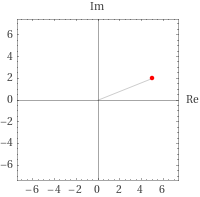
\includegraphics[width=0.25\textwidth]{argand.png} \\
        \text{The quadrant is $1$ the $\theta$ will remain the same as the ref $\angle$} \\
        \text{$\theta$ is $21.80^{\circ}$} \\
        \text{later below this section i will propose all the cases to work out $\theta$ due to different quadrant numbers} \\
        \text{The polar form of the complex number is:} \\
        5.39(\cos{(21.80)^{\circ}}+i\sin{(21.80)^{\circ}}) \\        
        \text{where $\theta$ is measured in degrees.} \\
    \end{split}
\end{equation}

\subsubsection{Working out $\theta$ in different quadrants}

Lets denote the quadrant number as $q_{n}$ and the ref angle as $\angle$.

\begin{equation}
    \theta =
    \left\{
        \begin{array}{lr}
            \angle, & \text{if } q_{1}\\
            180-\angle^{\circ}, & \text{if } q_{2} \\
            180+\angle^{\circ}, & \text{if } q_{3} \\
            360-\angle^{\circ}, & \text{if } q_{4} \\                        
        \end{array}
    \right\} 
\end{equation}

\chapter{De Moivre's Theorem}
\section{De Moivre's Theorem}
In mathematics, de Moivre's formula (also known as de Moivre's theorem and de Moivre's identity) states that for any real number x and integer n it holds that

    \begin{equation}
        (\cos{x}+i\sin{x})^{n} = \cos{n\cdot x}+i\sin{n\cdot x}
    \end{equation}

where $i$ is the imaginary unit. $i^2 = -1$ The formula is named after Abraham de Moivre, although he never stated it in his works.The expression $cosx + isinx$ is sometimes abbreviated to $cisx$.

The formula is important because it connects complex numbers and trigonometry. By expanding the left hand side and then comparing the real and imaginary parts under the assumption that $x$ is real, it is possible to derive useful expressions for $cosnx$ and $sinnx$ in terms of $cosx$ and $sinx$.

As written, the formula is not valid for non-integer powers $n$. However, there are generalizations of this formula valid for other exponents. These can be used to give explicit expressions for the nth roots of unity, that is, complex numbers $z$ such that $zn = 1$.

%insert image
\begin{figure}[h!]
    \centering
    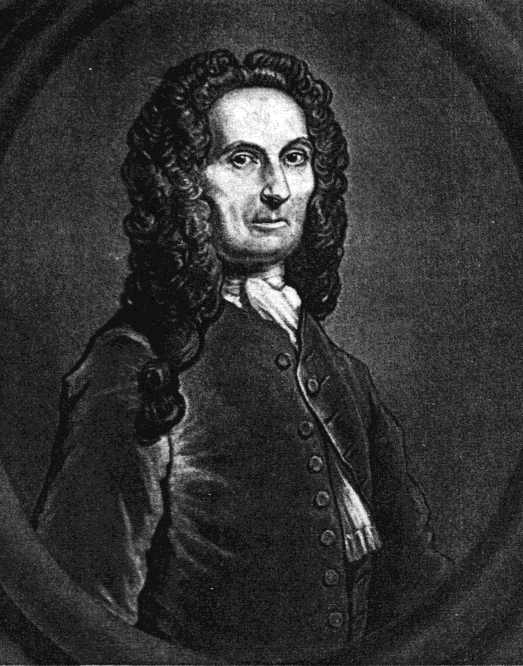
\includegraphics[width=0.5\textwidth]{demoivre.jpg}
    \caption{Abraham de Moivre a famous Mathematician}        
\end{figure}

\subsection{Combinations, and the Binomial Theorem}

Before moving on to the next section, let us try to understand the combinations and the Binomial Theorem.

\subsubsection{Factorials}

In mathematics, the factorial of a non-negative integer n, denoted by n!, is the product of all positive integers less than or equal to n. The factorial of n also equals the product of n with the next smaller factorial: For example, The value of 0! is 1, according to the convention for an empty product.


The factorial general equation is defined as:

\begin{equation}
     n! = n*(n-1)*(n-2)*...*1
\end{equation}

Example: 6!

    \begin{equation}
        6! = 6*5*4*3*2*1 = 720
    \end{equation}

Example: 3!

    \begin{equation}
        3! = 3*2*1 = 6
    \end{equation}

Example: 10!

    \begin{equation}
        10! = 10*9*8*7*6*5*4*3*2*1 = 3628800
    \end{equation}

%% draw a table of complex numbers i powers
%\begin{center}
%    \begin{tabular}{|c|c|}    
%        \hline	
%        $i$ & $\sqrt{-1}$ \\ \hline
%        $i^2$ & $-1$ \\ \hline
%        $i^3$ & $-i$ \\ \hline
%        $i^4$ & $1$ \\ \hline
%        $i^5$ & $i$ \\ \hline
%        $i^6$ & $-i$ \\ \hline
%        $i^7$ & $-1$ \\ \hline
%        $i^8$ & $i$ \\ \hline
%    \end{tabular}
%    \end{center}
%    
%    % describe table
%    \begin{center}
%        $i$ Chart.
%    \end{center}
%

% draw table of n and n!
\begin{center}
    \begin{tabular}{|c|c|}    
        \hline	
        $n$ & $n!$ \\ \hline
        $0$ & $1$ \\ \hline
        $1$ & $1$ \\ \hline
        $2$ & $2$ \\ \hline
        $3$ & $6$ \\ \hline
        $4$ & $24$ \\ \hline
        $5$ & $120$ \\ \hline
        $6$ & $720$ \\ \hline
        $7$ & $5040$ \\ \hline
        $8$ & $40320$ \\ \hline
        $9$ & $362880$ \\ \hline
        $10$ & $3628800$ \\ \hline
    \end{tabular}
    \end{center}
    
% describe table
\begin{center}
    Selected factorials.
\end{center}



\subsubsection{Combinations}

The formula for combinations is:
\begin{equation}
    C(n,k) = \frac{n!}{k!(n-k)!}
\end{equation}

where $n$ is the number of objects in the set and $k$ is the number of objects in the subset.
\linebreak
\linebreak
In mathematics, a combination is a selection of items from a set that has distinct members, such that the order of selection does not matter (unlike permutations). For example, given three fruits, say an apple, an orange and a pear, there are three combinations of two that can be drawn from this set: an apple and a pear; an apple and an orange; or a pear and an orange. More formally, a k-combination of a set S is a subset of k distinct elements of S. So, two combinations are identical if and only if each combination has the same members. (The arrangement of the members in each set does not matter.) If the set has n elements, the number of k-combinations, denoted as $C_{k}^{n}$ , is equal to the binomial coefficient

    \begin{equation}
        C_{k}^{n} = \binom{n}{k}
    \end{equation}

Example: Evaulating $C_{5}^{52}$


    
    \begin{equation}   
    \begin{split}     
        C_{5}^{52} = \binom{52}{5}  \\
        \binom{52}{5} = \frac{52!}{5!(52-5)!} \\
        \therefore C_{5}^{52} = 2598960
    \end{split}  
    \end{equation}

Example: Evaulating $C_{3}^{4}$

\begin{equation} 
    \begin{split}     
        C_{3}^{4} = \binom{4}{3}  \\
        \binom{4}{3} = \frac{4!}{3!(4-3)!} \\
        \therefore C_{3}^{4} = 4
    \end{split}
\end{equation}

\subsection{Binomial Theorem}

In elementary algebra, the binomial theorem (or binomial expansion) describes the algebraic expansion of powers of a binomial. According to the theorem, it is possible to expand the polynomial $(x + y)^n$ into a sum involving terms of the form $ax^{b}y^{c}$, where the exponents $b$ and $c$ are nonnegative integers with $b + c = n$, and the coefficient a of each term is a specific positive integer depending on $n$ and $b$.

The coefficient $a$ in the term of $ax^{b}y^{c}$ 
is known as the binomial coefficient $\binom{n}{b}$ or $\binom{n}{c}$ 
the two have the same value. 
These coefficients for varying $n$ and $b$ can be arranged to form Pascal's triangle. 
These numbers also occur in combinatorics, where $\binom {n}{b}$ 
gives the number of different combinations of $b$ elements that can be chosen from an $n$-element set. 
Therefore $\binom{n}{b}$ is often pronounced as $n$ choose $b$".

%draw pascals triangle

\begin{center}
\begin{tabular}{rccccccccc}
    $n=0$:&    &    &    &    &  1\\\noalign{\smallskip\smallskip}
    $n=1$:&    &    &    &  1 &    &  1\\\noalign{\smallskip\smallskip}
    $n=2$:&    &    &  1 &    &  2 &    &  1\\\noalign{\smallskip\smallskip}
    $n=3$:&    &  1 &    &  3 &    &  3 &    &  1\\\noalign{\smallskip\smallskip}
    $n=4$:&  1 &    &  4 &    &  6 &    &  4 &    &  1\\\noalign{\smallskip\smallskip}    
\end{tabular}
\end{center}

\begin{center}
    Pascal's Triangle
\end{center}

using Pascal's Triangle, lets draw a table for $(x+y)^n$

    \begin{center}
    \begin{tabular}{|c|c|}    
        \hline	
        $n$ & $(x + y)^n$ \\ \hline
        $0$ & $1$ \\ \hline
        $1$ & $x+y$ \\ \hline
        $2$ & $x^2+2xy+y^2$ \\ \hline
        $3$ & $x^3+3x^2y+3xy^2+y^3$ \\ \hline
        $4$ & $x^4+4x^3y+6x^2y^2+4xy^3+y^4$ \\ \hline
        $5$ & $x^5+5x^4y+10x^3y^2+10x^2y^3+5xy^4+y^5$ \\ \hline
 
    \end{tabular}
    \end{center}

and thats how we use Pascal's Triangle to evaluate any binomial expansion. \newline

Now let us use the binomial theorem formula to evaluate $(x+y)^n$

First lets describe the binomial formula
The formula is for any $(x+y)^n$:
\begin{equation}
    (x+y)^n = \sum_{k=0}^{n} \binom{k}{n}x^{n-k}y^k
\end{equation}

Example: Using the binomial theorem to evaluate $(x+y)^2$

\begin{equation}
    \begin{split}
        (x+y)^2 = \sum_{k=0}^{2} \binom{2}{k}x^{2-k}y^k \\
        = \binom{2}{0}x^{2} + \binom{2}{1}x^{1}y + \binom{2}{2}x^{0}y^2 \\
        \therefore (x+y)^2 = x^2 + 2xy + y^2
    \end{split}    
\end{equation}

Example: Using the binomial theorem to evaluate $(x+y)^3$
\begin{equation}
    \begin{split}
        (x+y)^3 = \sum_{k=0}^{3} \binom{3}{k}x^{3-k}y^k \\
        = \binom{3}{0}x^{3} + \binom{3}{1}x^{2}y + \binom{3}{2}x^{1}y^2 + \binom{3}{3}x^{0}y^3 \\
        \therefore (x+y)^3 = x^3+3x^2y+3xy^2+y^3
    \end{split}
\end{equation}

we can now proceed to learning De Moivre's theorem now :-)

\subsection{Expressing $\cos{n\theta} $ and $sin{n\theta}$ in terms of powers of $\cos{\theta}$ and $\sin{\theta}$}

Now the method of De Moivre's theorem is to express the trigonometric functions in terms of powers of the cosine and sine.

if we remember De Moivre's theorem, it is given that:

\begin{equation}
    \begin{split}
        (\cos{\theta}+i\sin{\theta})^n = {\cos{n\theta}+i\sin{n\theta}} \\
    \end{split}
\end{equation}

but we can not use the formula above to express $(\cos{n\theta}+i\sin{n\theta})^n$ in terms of powers of $\cos{\theta}$ and $\sin{\theta}$

our methodology is that we must implement the binomial theorem equate the real part to the cosine and the imaginary part to the sine.   

    \begin{equation}
        \begin{split}
            (\cos{\theta}+i\sin{\theta})^n = \binom{n}{k}(cos{\theta})^{n-k}(isin{\theta})^{k} \\  
            \therefore \text{from De Moivre}  (\cos{n\theta}+i\sin{n\theta}) = \binom{n}{k}(cos{\theta})^{n-k}(isin{\theta})^{k} \\
        \end{split}
    \end{equation}

Example working out $\cos{4\theta},sin{4\theta}$:

    \begin{equation}
        \begin{split}
            (\cos{\theta}+i\sin{\theta})^4 = \binom{4}{k}(cos{\theta})^{4-k}(isin{\theta})^{k} \\            
            = \cos ^4\left(x\right)+4i\cos ^3\left(x\right)\sin \left(x\right)-6\cos ^2\left(x\right)\sin ^2\left(x\right)-4i\sin ^3\left(x\right)\cos \left(x\right)+\sin ^4\left(x\right) \\
            \text{factoring real and imaginary parts} \\
            \left(\cos ^4\left(x\right)-6\cos ^2\left(x\right)\sin ^2\left(x\right)+\sin ^4\left(x\right)\right)+\left(4\cos ^3\left(x\right)\sin \left(x\right)-4\sin ^3\left(x\right)\cos \left(x\right)\right)i \\            
            \therefore \cos{4\theta} = \cos ^4\left(x\right)-6\cos ^2\left(x\right)\sin ^2\left(x\right)+\sin ^4\left(x\right) \\
            \therefore \sin{4\theta} = 4\cos ^3\left(x\right)\sin \left(x\right)-4\sin ^3\left(x\right)\cos \left(x\right) \\
        \end{split}
    \end{equation}

\subsection{Determining $\cos^n{\theta}$ and $\sin^n{\theta}$ using De Moivre's Theorem}

First lets work out an expression for $(\cos{\theta}+i\sin{\theta})^n+ (\cos{\theta}+i\sin{\theta})^{-n}$ where $\forall{n} \in \mathbb{N}$ 

\begin{equation}
    \begin{split}
        \text{let $z=\cos{\theta}+i\sin{\theta}$} \\
        \text{then $z^n=(\cos{\theta}+i\sin{\theta})^n$} \\
        \text{also $z^{-n}=(\cos{\theta}+i\sin{\theta})^{-n}$} \\                            
        \text{now we work out what $z^n$+$z^{-n}$ is} \\
        = (\cos{\theta}+i\sin{\theta})^n+ (\cos{\theta}+i\sin{\theta})^{-n} \\        
        = \cos{(ne)}+i\sin{(ne)}+\cos{(-ne)}+i\sin{(-ne)} \\
        = \cos{(ne)}+i\sin{(ne)}+\cos{(ne)}-i\sin{(ne)} \\
        = 2cos{(ne)} \\
        \therefore z^{n}+z^{-n} = 2\cos{ne} \\
        \text{rewriting this expression can be seen as $(z+z^{-1})^n = (2cos\theta)^n$}\\        
        \land (z-z^{-1})^n = (2i\sin{\theta})^n \\ 
    \end{split}
\end{equation}

Example: Determining $\cos^3{\theta}$

\begin{equation}
    \begin{split}
        (2\cos{\theta})^3 = (z+z^{-1})^3 \\
        \text{LHS} = 8\cos^3{(\theta)} \\
        \text{RHS} = z^3+3z+3z^{-1}+z^{-3} \\
        \text{now we factor in terms by $z^n$+$z^{-n}$} \\ 
        \text{RHS} = 3(z+z^{-1}) + (z^{3}+z^{-3}) \\
        \text{RHS} = 6cos{\theta}+2cos{3\theta} \\
        8cos^{3}\theta = 6cos{\theta}+2cos{3\theta} \\
        cos^{3}\theta = \frac{3}{4}\cos{\theta}+\frac{1}{4}\cos{3\theta} \\
    \end{split}
\end{equation}

Example: Determining $\sin^4{\theta}$

\begin{equation}
    \begin{split}
        (2i\sin{\theta})^4 = (z-z^{-1})^4 \\
        \text{LHS} = 16i^{4}\sin^4{(\theta)} \\         
        \text{RHS} = \sum _{i=0}^4\binom{4}{i}z^{\left(4-i\right)}\left(-z^{-1}\right)^i \\
        \text{RHS} = z^4-4z^2+6-\frac{4}{z^2}+\frac{1}{z^4} \\
        \text{RHS} = z^{4}-4z^{2}+6-4z^{-2}+z^{-4} \\
        \text{now we factor in terms by $z^n$+$z^{-n}$} \\ 
        \text{RHS} = (z^4+z^{-4})-4(z^2+z^{-2})+6 \\
        \text{RHS} = 2\cos{4\theta}-8\cos{2\theta}+6 \\
        16\sin^4{(\theta)} =  2\cos{4\theta}-8\cos{2\theta}+6  \\
        \text{now we can see that the expression is} \\
        sin^{4}\theta = \frac{1}{8}\cos{4\theta}-\frac{1}{2}\cos{2\theta}+\frac{3}{8}\\
    \end{split}
\end{equation}

\subsection{Finding the $n^{th}$ roots of a complex number}

Let us consider the standard form of a complex number $a+bi$ and polar form $r(\cos{\theta}+i\sin{\theta})$

Methodology:
\begin{equation}
    \begin{split}    
        a+bi = r\cos{\theta}+i\sin{\theta} \\
        \text{let $r=\sqrt{a^2+b^2}$} \\
        \text{let $\theta=\arctan\left(\frac{b}{a}\right)$} \\ 
        a+bi = rcis{\theta} \\
        a+bi = re^{i\theta} \text{ (Euler's)} \\
        re^{i\theta} = re^{i(\theta+2\pi*k)} \text {, $k$} \in \mathbb{Z} \\
        (a+bi)^{\frac{1}{n}}= (re^{i(\theta+2\pi*k)})^{\frac{1}{n}} \\
        (re^{i(\theta+2\pi*k)})^{\frac{1}{n}} = r^{\frac{1}{n}}e^{i(\frac{\theta+2\pi*k}{n})} \\
        \text{where}  \\
        k=0 : \frac{\theta}{n} \\ 
        k=1 : \frac{\theta}{n}+\frac{2\pi}{n}*1 \\
        k=2 : \frac{\theta}{n}+\frac{2\pi}{n}*2 \\
        \vdots  \\
        k=n : \frac{\theta}{n}+\frac{2\pi}{n}*n  \\    
        = \frac{\theta}{n}+2\pi \\
        \therefore (a+bi)^{\frac{1}{n}}= r^{\frac{1}{n}}e^{i(\frac{\theta+2\pi*k}{n})} \text{ , } k=0,1,\ldots,n-1 \\
        \text{ or } (a+bi)^{\frac{1}{n}}=r^{\frac{1}{n}}cis{(\frac{\theta+2\pi*k}{n})} \text{ , } k=0,1,\ldots,n-1 \\
    \end{split}
\end{equation}

Example: Finding cube root of $\frac{-27\sqrt{2}}{2}+\frac{27\sqrt{2}}{2}i$

\begin{equation}
    \begin{split}
        \text{Lets solve $r$, $\theta$} \\
        % find r (modulus) %  
        \text{let $r=\sqrt{a^2+b^2}$} \\
        \text{let $\theta=\arctan\left(\frac{b}{a}\right)$} \\
        r = \sqrt{(\frac{-27\sqrt{2}}{2})^2+(\frac{27\sqrt{2}}{2})^2} = 27\\
        \theta = \arctan(-1) = \pi-\frac{1}{4}\pi = \frac{3\pi}{4} \text{ since $\theta$ falls in quadrant 2} \\
        \text{now we can find the cube root using our definition} \\        
        (a+bi)^{\frac{1}{3}}= 27^{\frac{1}{3}}cis{(\frac{\frac{3\pi}{4}+2\pi*k}{3})} \text{ , } k=0,\ldots,2 \\
        k=0 : 3cis{(\frac{\pi}{4})} \\
        k=1 : 3cis{(\frac{\pi}{4}+\frac{2\pi}{3})} = 3cis{(\frac{11\pi}{12})} \\
        k=2 : 3cis{(\frac{\pi}{4}+\frac{4\pi}{3})} = 3cis{(\frac{19\pi}{12})} \\        
    \end{split}
\end{equation}

\newpage

\end{document}
